\section{System model and problem}
\label{sec:Problem description}
In this section, we first introduce  basic concepts on virtual network embedding, then present our survivable virtual network embedding problem.


\subsection{Virtual network embedding}


We represent a \textbf{virtual network} (VN) as an undirected graph $G (V,E)$ where $V$ and  $E$ are the sets of virtual nodes and virtual links, respectively. Each virtual link $e_{ij}$ has the bandwidth demand $d_{ij}$. Each virtual node  $v_i$ has the computation capacity demand   $d_i$. For virtual node $v_i$, the virtual function required to be executed on the virtual node is denoted as $f(i)$. Fig.\ref{fig:VNQSNVNE}(a) shows an example virtual network with virtual node set $V=\{v_1,v_2,v_3,v_4\}$ and virtual edge set $E= \{e_{12},e_{13},e_{14},e_{23}\}$. The virtual functions required to be executed on these virtual nodes are  $f(1)=f_1$, $f(2)=f_2$, $f(3)=f_3$, $f(4)=f_4$, respectively.
%\begin{figure}
%\centering
%\begin{minipage}[t]{0.45\linewidth}
%% Requires \usepackage{graphicx}
%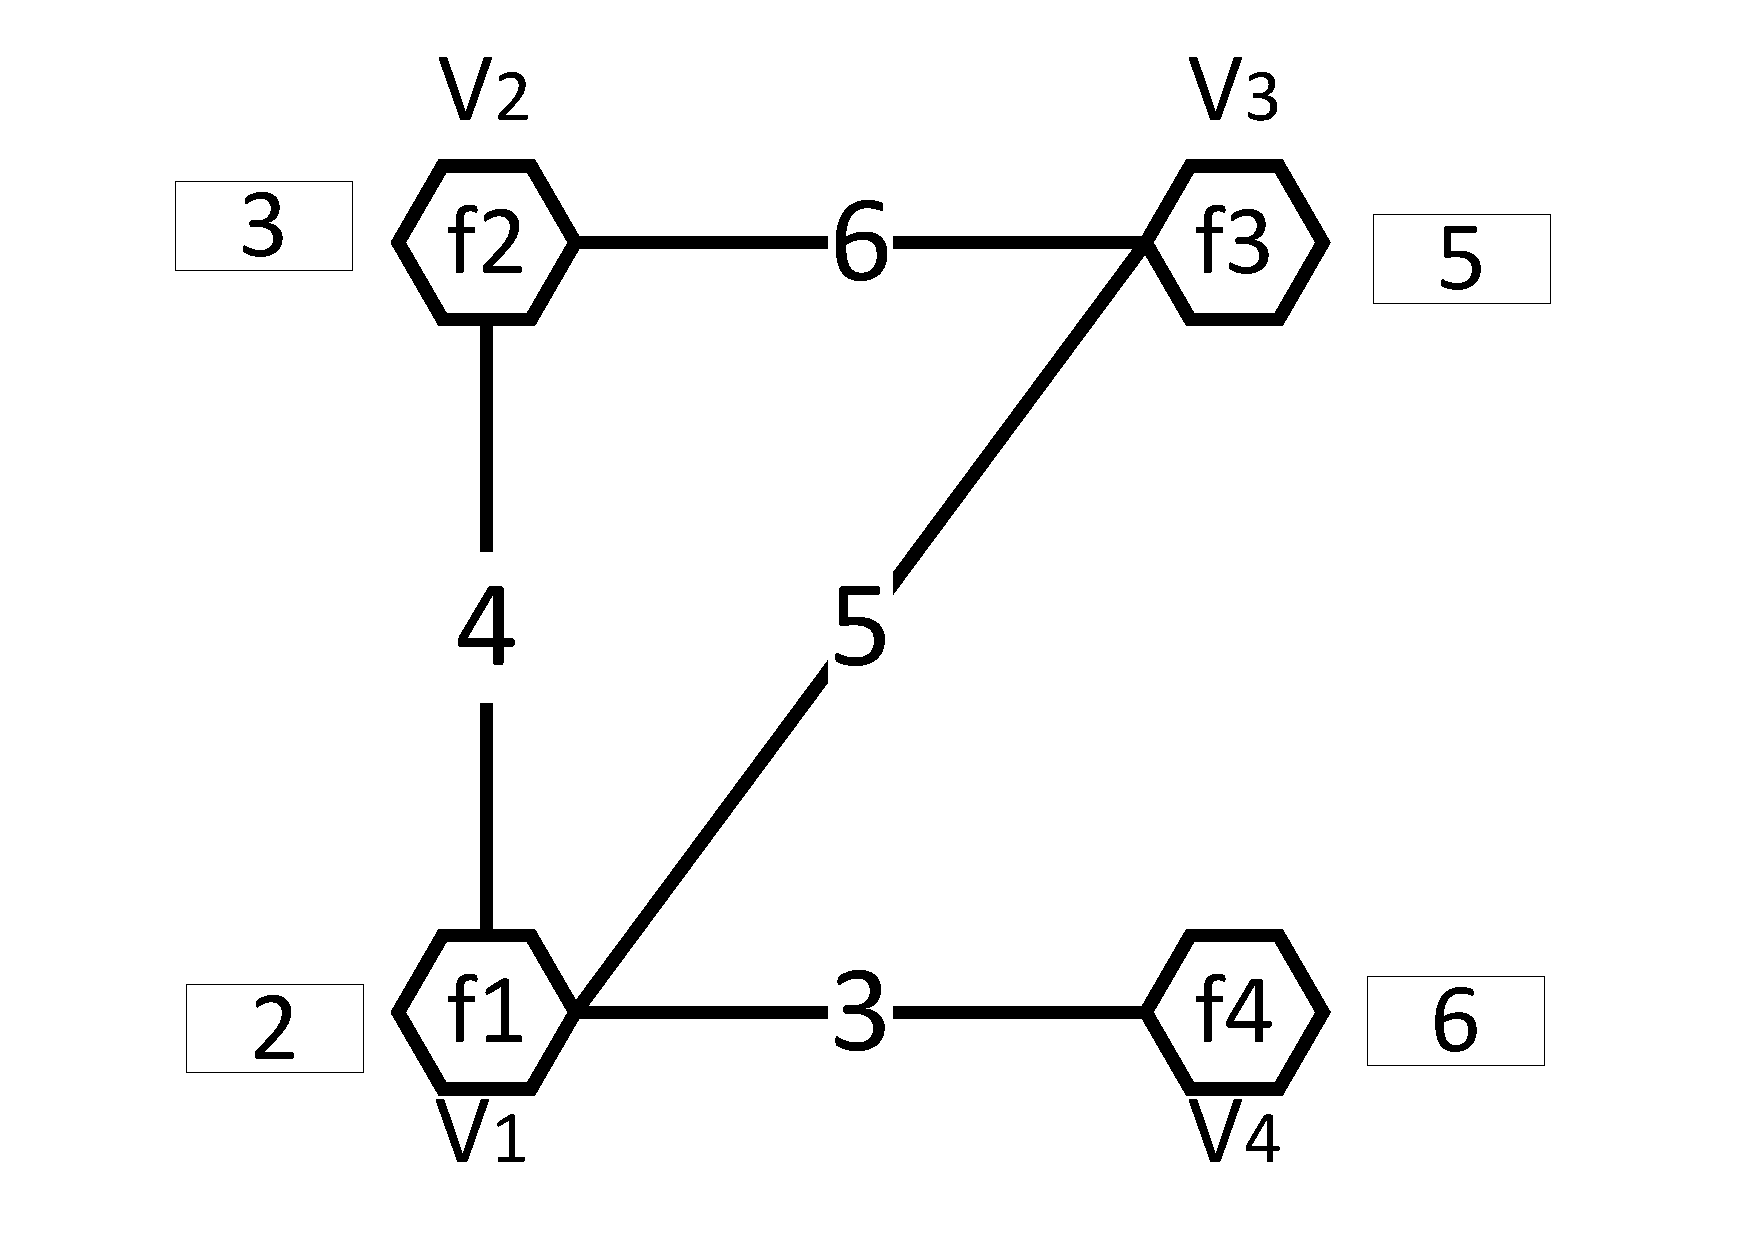
\includegraphics[width=1.3in]{Fig/VNQ}\\
%\caption{Virtual Network Request $G(V,E)$, $V=\{v_1,v_2,v_3,v_4\}$, $E=\{e_{12},e_{23},e_{13},e_{14}\}$,  $f^V=\{f_1,f_2,f_3,f_4\}$, $d_i=\{2,3,5,6\}$, $d_{ij}=\{4,5,3,6\}.$}\label{fig:VNQ}
%\end{minipage}
%\hfill
%\begin{minipage}[t]{0.45\linewidth}
%% Requires \usepackage{graphicx}
%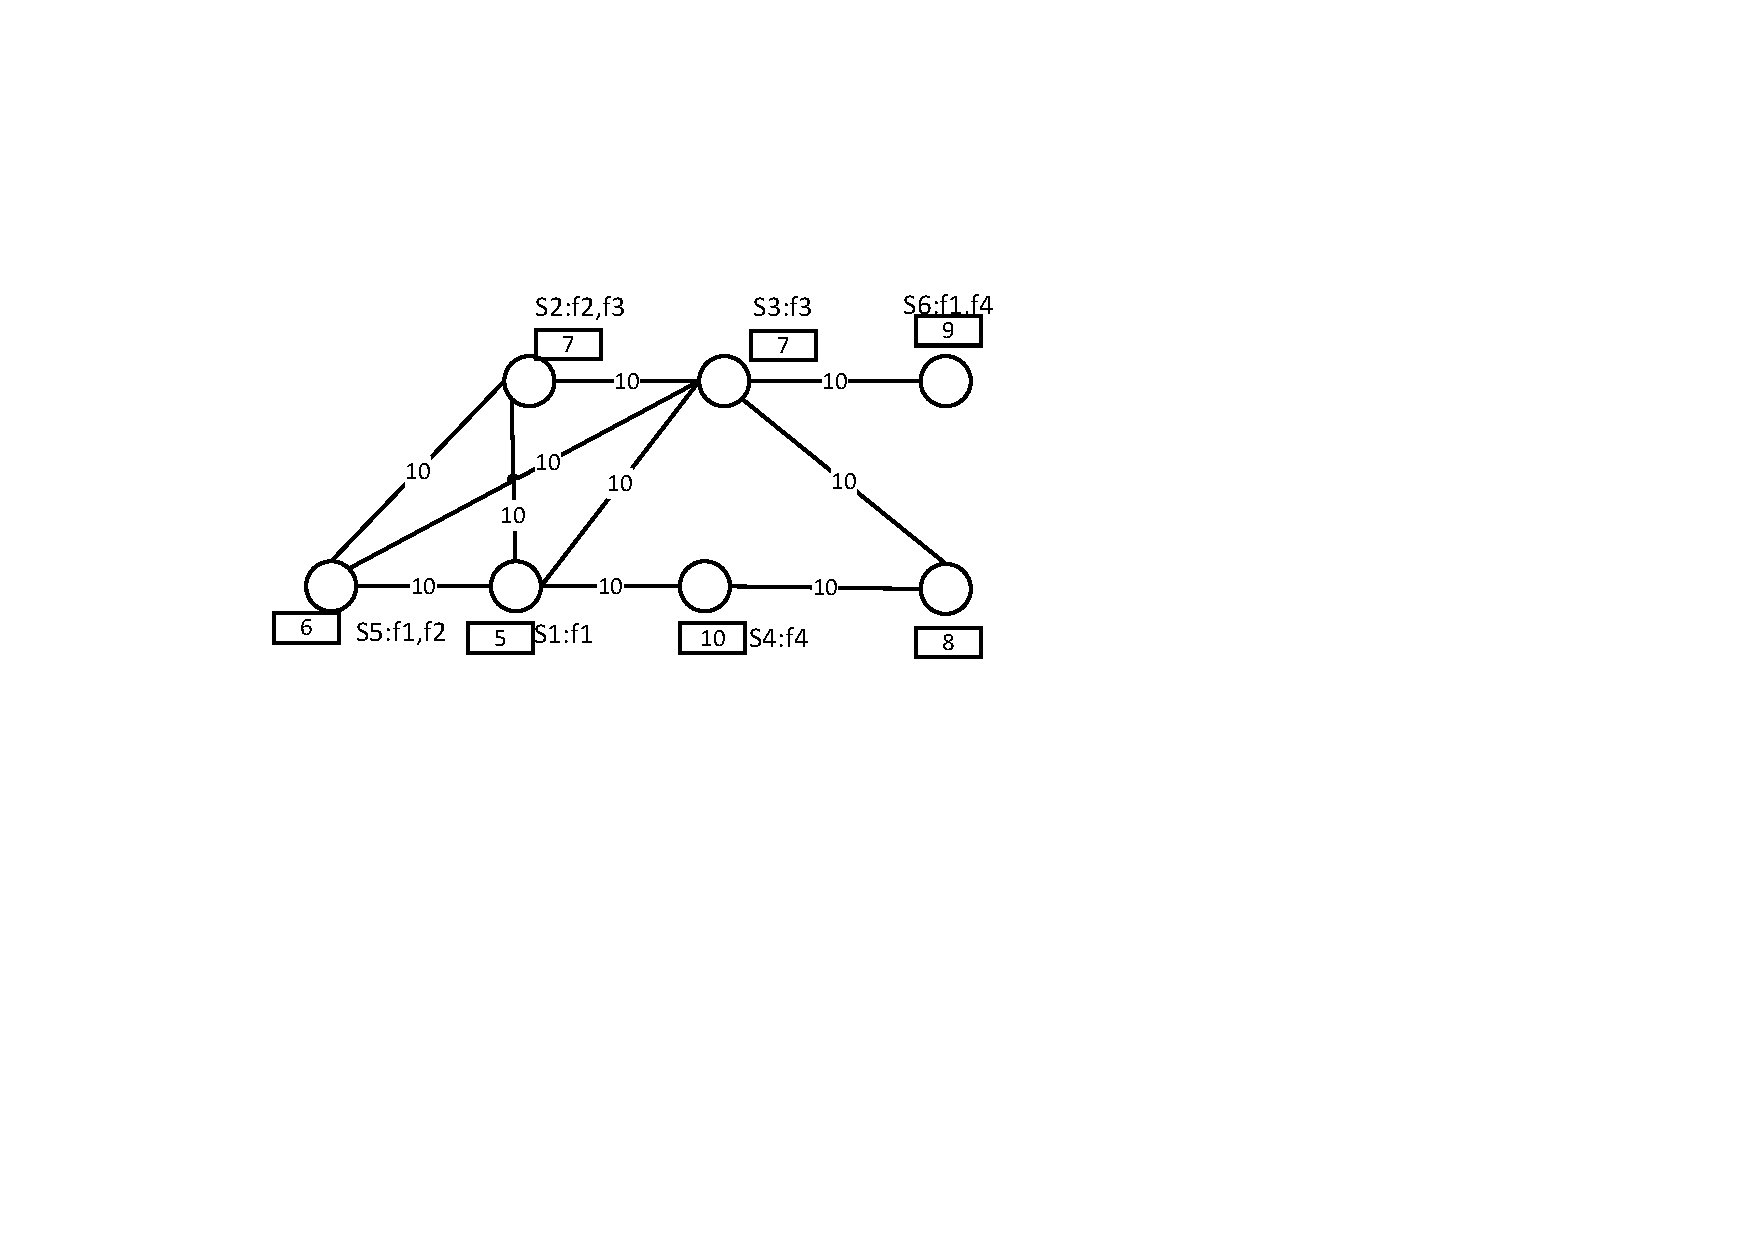
\includegraphics[width=1.8in]{Fig/SN}\\
%\caption{Physical Network $G^S(V^S,E^S), V^S=\{s_1,s_2,s_3,s_4,s_5,s_6,s_7\}, E^S=\{l_{12},l_{13},l_{14},l_{15},l_{23},l_{25},l_{35},l_{36},l_{37},l_{47}\}, F^S=\{\{f_1\},\{f_2,f_3\},\{f_3\},\{f_4\},\{f_1,f_2\},\{f_1,f_4\},\{f_2,f_3\}\}, c_i=\{5,7,7,10,6,9,8\}, %b_{ij}=\{10,10,10,10,10,10,10,10,10,10\}$}\label{fig:SN}
%\end{minipage}
%\end{figure}

\begin{figure*}
\centering
% Requires \usepackage{graphicx}
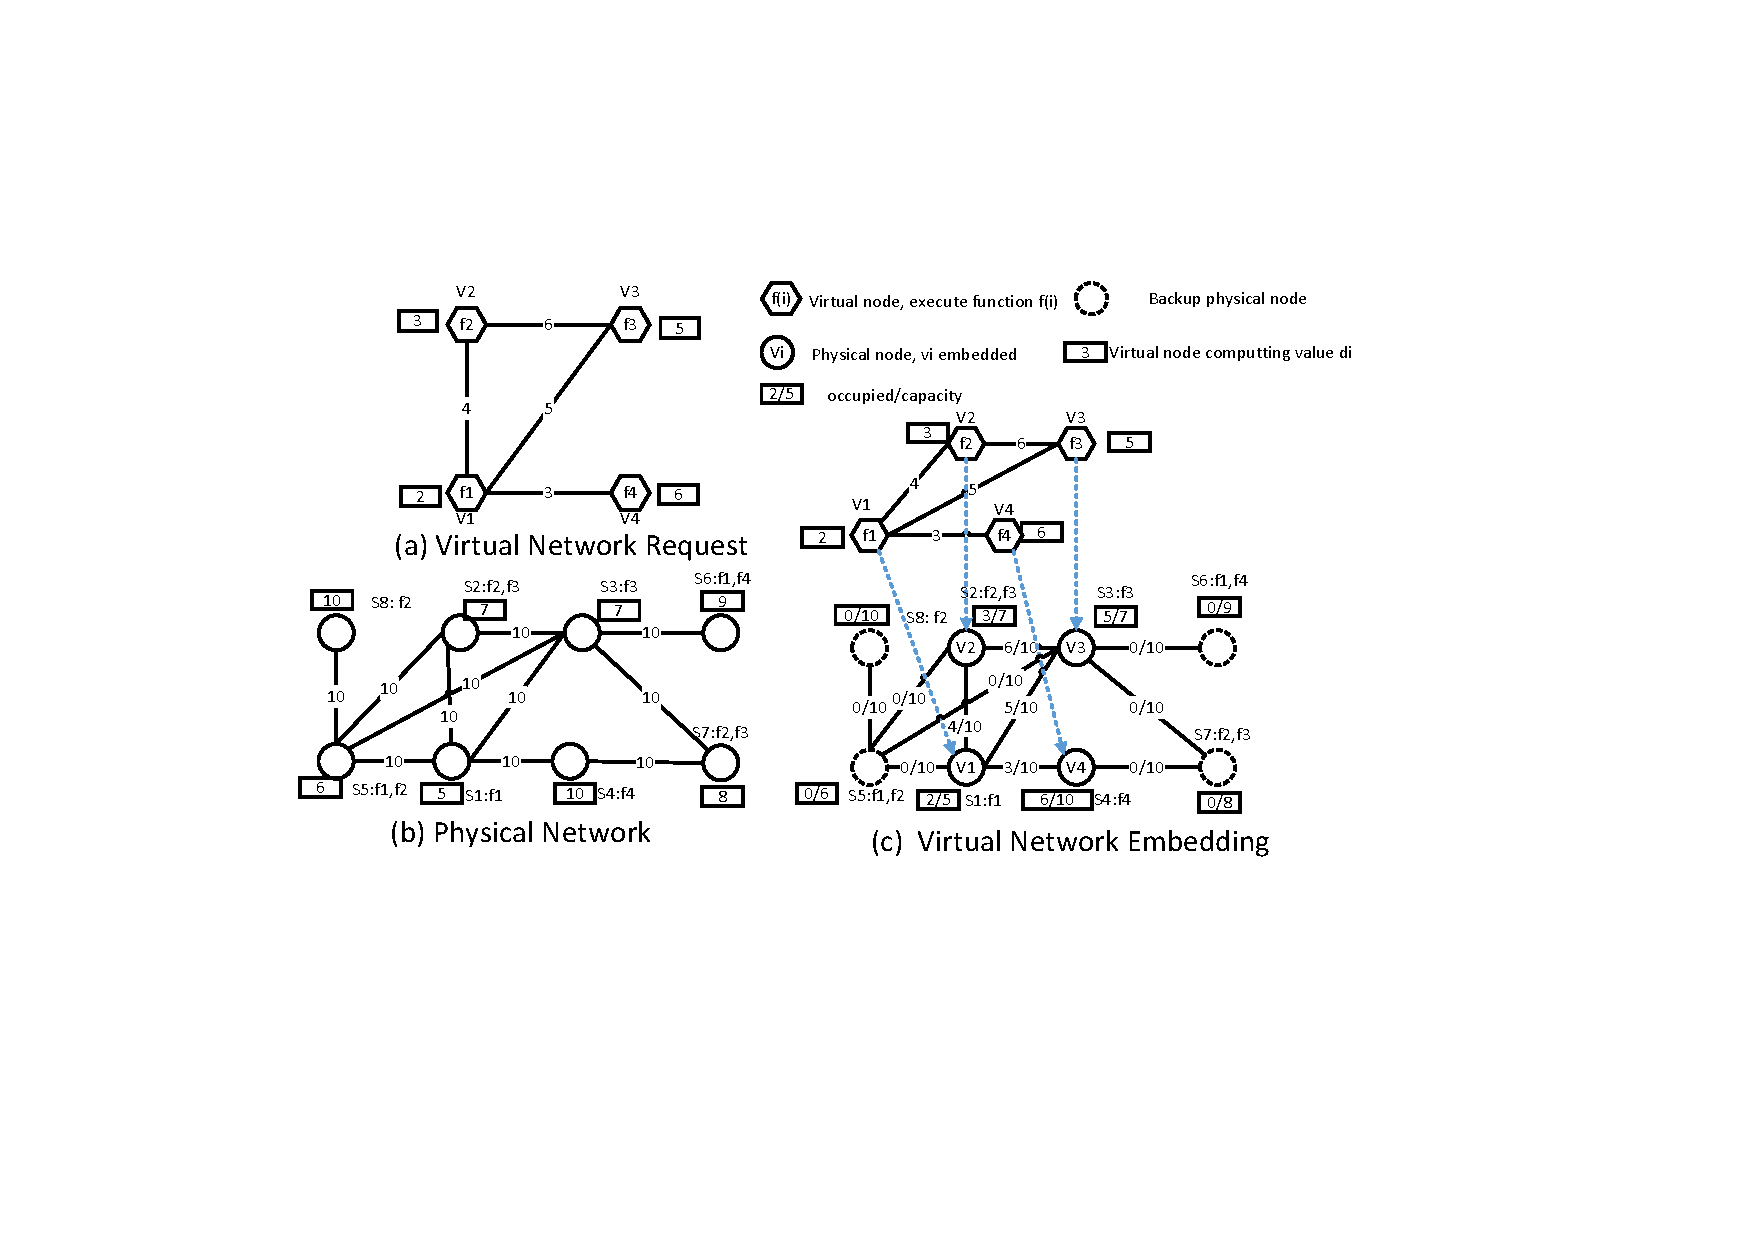
\includegraphics[width=5in]{Fig/VNQSNVNE}\\
\caption{(a) Virtual Network Request $G(V,E)$, $V=\{v_1,v_2,v_3,v_4\}$, $E=\{e_{12},e_{23},e_{13},e_{14}\}$,  $f(i)=\{f_1,f_2,f_3,f_4\}$, $d_i=\{2,3,5,6\}$, $d_{ij}=\{4,5,3,6\}. $(b) Physical Network $G(S,L), S=\{s_1,s_2,s_3,s_4,s_5,s_6,s_7,s_8\}, L=\{l_{12},l_{13},l_{14},l_{15},l_{23},l_{25},l_{35},l_{36},l_{37},l_{47},l_{58}\}, F(i)=\{\{f_1\},\{f_2,f_3\},\{f_3\},\{f_4\},\{f_1,f_2\},\{f_1,f_4\},\{f_2,f_3\},\{f_2\}\}, c_i=\{5,7,7,10,6,9,8,10\}, b_{ij}=\{10,10,10,10,10,10,10,10,10,10,10\}$ (c) Vertex mapping $v_1\rightarrow s_1, v_2\rightarrow s_2, v_3\rightarrow s_3, v_4\rightarrow s_4$, link mapping $e_{12}\rightarrow l_{12},e_{23}\rightarrow l_{23},e_{13}\rightarrow l_{13},e_{14}\rightarrow l_{14}$.}\label{fig:VNQSNVNE}
\end{figure*}


We model the \textbf{physical network} as an undirected graph $G (S,L)$, where $S$ and $L$ is the sets of physical nodes and physical links, respectively.
 For physical node  $s_i$, we use $F(i)$ and $c_i$ to respectively denote the set of feasible virtual functions can be executed on this node and the available computational capacity. Each physical link $l_{ij}$ has an available bandwidth of $b_{ij}$. In  the physical network in Fig.\ref{fig:VNQSNVNE}(b), physical node set $S=\{s_1,s_2,s_3,s_4,s_5,s_6,s_7,s_8\}$,  link set $L=\{l_{12},l_{13},l_{14},l_{15},l_{23},l_{25},l_{35},l_{36},l_{37},l_{47},l_{58}\}$, the  feasible virtual function set of each physical node is  $F(1)=\{f_1\}$, $F(2)=\{f_2,f_3\}$, $F(3)=\{f_3\}$, $F(4)=\{f_4\}$, $F(5)=\{f_1,f_2\}$, $F(6)=\{f_1,f_4\}$, $F(7)=\{f_2,f_3\}$,$F(8)=\{f_2\}$, respectively.



Given the VN request $G (V,E)$, the problem of \textbf{\emph{virtual network embedding}} aims to map this request onto the physical network $G (S,L)$ while providing enough resource as demanded. A feasible mapping should satisfy three constraints including node capacity constraint, link bandwidth constraint, and function type constraint.

For a virtual node $v_i$, a physical node $s_j$ can hold this virtual node only when both node capacity constraint  and  function type constraint (i.e., ${f_i} \in {F_j}$) are satisfied, that is, the node capacity request should be satisfied by the physical node with $d_i\leq c_j$, the virtual function required to be executed on  virtual node ${v_i}$ can be executed on physical node $s_j$ with ${f_i} \in {F_j}$. If a physical node $s_j$ satisfies both two  constraints, the node mapping is feasible, and we denote such mapping as $\phi ({v_i}) = {s_j}$.

%Denote the corresponding physical node that holds $v_i$ as $s_j$. Under node capacity constraint, we have $d_i\leq c_j$, that is, the node capacity request should be satisfied by the physical node. Besides capacity constraint, there is a location constraint should be satisfied on the physical node, that is, a virtual node ${v_i} \in V$ can only be provisioned on a physical node $s_j$ with ${f_i} \in {F_j}$. That is, the virtual function running on virtual node ${v_i}$ can be executed on physical node $s_j$. If a physical node $s_j$ satisfies both node capacity constraint and location constraint, the node mapping is feasible, and we denote such mapping as $\phi ({v_i}) = {s_j}$.

For a virtual link $e_{ij}$ with its two virtual nodes are mapped to two physical nodes $s_{i'}$ and $s_{j'}$ (i.e., $\phi({v_i}) = {s_{i'}}$ and $\phi({v_j}) = {s_{j'}}$). Under link bandwidth constraint, if $d_{ij}\leq b_{i'j'}$ where $b_{i'j'}$ is the  available bandwidth  of the path connecting the physical nodes $s_{i'}$ and $s_{j'}$, virtual link  $e_{ij}$ can be mapped to the physical path $p_{\phi({v_i}) \phi({v_j})}$, we denote the feasible link mapping as $\rho(e_{ij}) = p_{\phi({v_i}) \phi({v_j})}$.

Obviously, to find a feasible virtual network embedding, we should find two mapping functions $\phi$ and $\rho$ to map all the virtual nodes to physical nodes, and all the virtual links to physical paths.


Fig.\ref{fig:VNQSNVNE}(c) shows a feasible virtual network embedding to embed virtual network in Fig.\ref{fig:VNQSNVNE}(a) to the physical network in Fig.\ref{fig:VNQSNVNE}(b) where  virtual node $v_1$ is embedded in physical node $s_1$, virtual node $v_2$ is embedded in physical node $s_2$, virtual node $v_3$ is embedded in physical node $s_3$, and virtual  node $v_4$ is embedded in physical node $s_4$, respectively. In Fig.\ref{fig:VNQSNVNE}(C), we also show the resource occupied and available in the physical network after such mapping. For example, for physical node $s_1$, its occupied computation capacity is 2 and the available capacity is 5. %The virtual link $e_{12}$ is mapped to physical link $l_{12}$ , we also draw the occupied bandwidth and the available bandwidth along the physical link  $l_{12}$.


%, we embed virtual network request as shown in Fig.\ref{fig:VNQSNVNE}(A) into the substrate network, node $v_1$ is embedded in node $s_1$, node $v_2$ is embedded in node $s_2$, node $v_3$ is embedded in node $s_3$, node $v_4$ is embedded in node $s_4$.  node computing demand of every virtual node is not more than these virtual nodes corresponding substrate node's remain node computing. Every link of virtual network request exist a corresponding path consisted of substrate node and remain bandwidth of all links of corresponding path is more than demand  bandwidth of the virtual network link.


Given the VN request $G (V,E)$ and the physical network  $G (S,L)$, for a feasible mapping, we  denote the mapping physical graph as $G\left( {\hat S,P} \right)$ where $\hat S$ is the physical node set that hold the virtual nodes with $\hat S = \{ {s_{i'}}:\phi({v_i}) = {s_{i'}},for\ {\rm{ }}all\ {v_i} \in V,{s_{i'}} \in S\}$  and $P$ is the path set in which each holds one virtual link with $P = \{ p_{\phi({v_i}) \phi({v_j})}:\rho(e_{ij}) = p_{\phi({v_i}) \phi({v_j})}{\rm{ }}, for\ all,{e_{ij}} \in E\}$. As each virtual link corresponds a physical network path which consisting of multiple physical links, we also denote $G\left( {\hat S,\hat L} \right)$ as the occupying physical network with  $\hat L = \{ {l_{pg}}:{l_{pg}} \in {p_{s_{i'}s_{j'}}}, \rho(e_{ij}) = p_{\phi({v_i}) \phi({v_j})},for\ all\ {e_{ij}} \in E,{l_{pg}} \in L\}$.

 %only subset of $S$ and $L$ are involved to hold the virtual network. We denote the sub-graph as $G\left( {\hat S,\hat L} \right)$ where $\hat S$ is the subset of $S$ and $\hat L$ is the subset of $L$. Obviously, we have $\hat S = \{ {s_{i'}}:{v_i} \to {s_{i'}}{\rm{ }}for{\rm{ }}all{\rm{ }}{v_i} \in V,{s_{i'}} \in S\}$ and $\hat L = \{ {l_{pg}}:{l_{pg}} \in {p_{i'j'}},{e_{ij}} \to {p_{i'j'}}{\rm{ }}for{\rm{ }}all{\rm{ }}{e_{ij}} \in E,{l_{pg}} \in L\}$. We denote $G\left( {\hat S,\hat L} \right)$ as the occupying physical network of the virtual request. As ${e_{ij}} \to {p_{i'j'}}$, that is, each virtual link corresponding a path, we can also denote the mapping physical graph as $G\left( {\hat S,P} \right)$  where $P$ is the corresponding path sets in the process of the embedding mapping.




Lots of studies investigate the virtual network embedding problem \cite{fischer2013virtual}, as the focus of this paper is not virtual network embedding, we adopt algorithm in \cite{lischka2009virtual} as the basic virtual network embedding algorithm.
%There has existed most studies about virtual network embedding method listed in a survey paper\cite{fischer2013virtual}.


\subsection{Survivable virtual network embedding}
Due to malicious attacks, natural disasters, unintentional cable cuts, planned maintenance, equipment malfunctioning, physical nodes that host the virtual nodes may suffer unavoidable fail. Failure in the VN can happen when single or multiple physical network components failures, which results in financial losses. In general, the multiple physical node's simultaneous failure is mutual independent, a single node failure happen at most of time\cite{yeow2011designing}. In this paper, we study the survivable virtual network embedding problem with single node failure. In section, we will discuss how our algorithm can be extended to the scenario with multiple node failure.


For a VN request $G (V,E)$ and a physical network $G (S,L)$, given a feasible mapping with its occupying physical network $G\left( {\hat S,\hat L} \right)$, this paper wants to add minimum backup physical resources to  provide survivable network service when any one physical node fails.

\begin{figure}
\centering
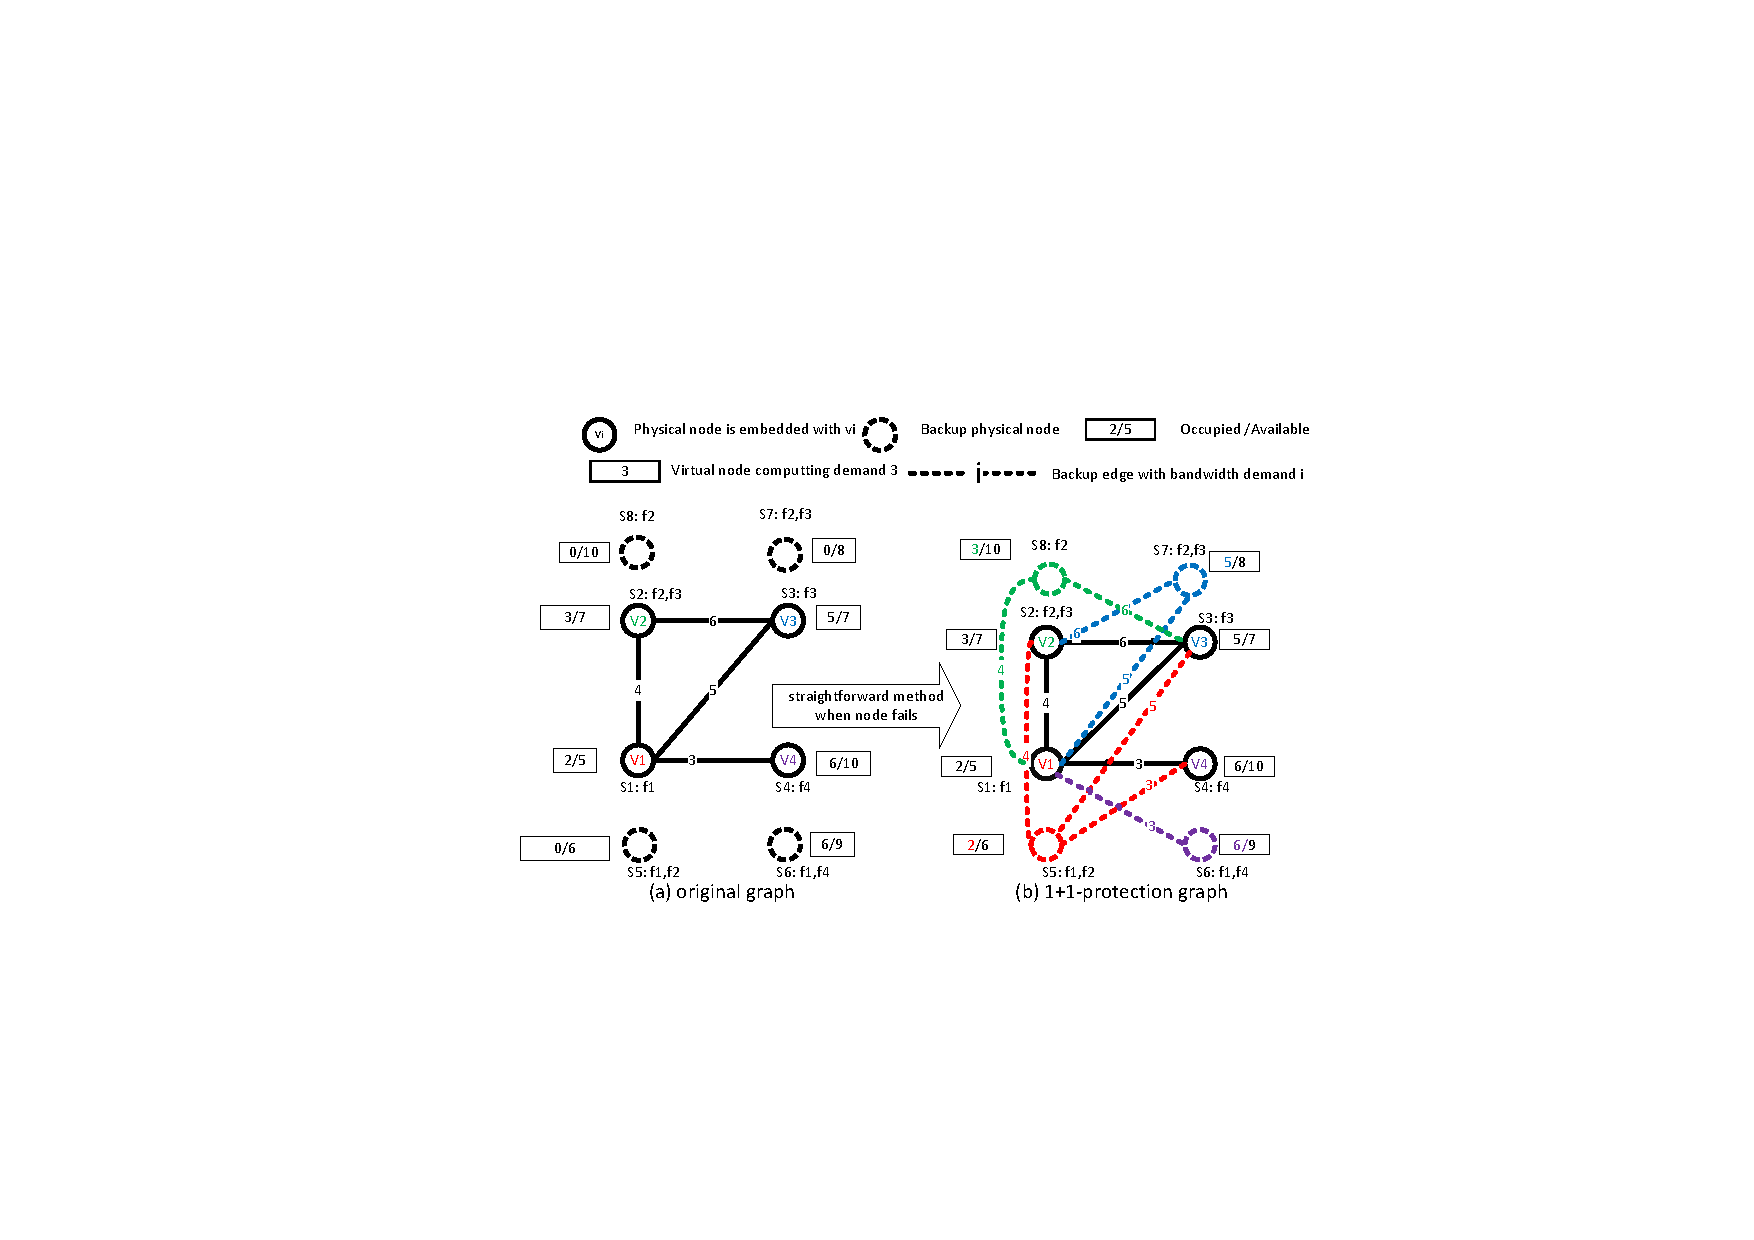
\includegraphics[width=3.5in]{Fig/One2OneProtection}\\
\caption{1+1-protection scheme}\label{fig:One2OneProtection}
\end{figure}

Node failures not only affect the visualized services running on the failed physical node, but also would terminate all the communications which traverse through this node. The fail of physical node $ {s_i} \in S $ results in the fail of physical links in ${L_i} = \left\{ {{l_{ik}}:k \in N(i)} \right\}$  where ${N(i)}$ is the neighbor nodes of node $ {s_i} $.

As we can not predict which node will fail even though we know multiple nodes will not simultaneously fail, to handle single node failure, one straightforward way  is to provision dedicated backup resource for each virtual node  in a VN request, also known as the 1 + 1-protection scheme.  Fig.\ref{fig:One2OneProtection} utilizes an example to illustrate this straightforward way. In the example, a virtual network with  4 virtual nodes are mapped to a physical network, where 4 physical nodes are involved in such embedding. To provide 1 + 1-protection scheme,  4 backup nodes, 8 backup links are added in the graph.

Although 1 + 1-protection scheme is simple to implement, it requires large amount of  backup resource. The aim of this paper is to provide survival network service with minimum backup resource cost.


%For example, when node $s_2$ fails, as it runs function $f_2$ for $v_2$ in the VN network, 1 backup node $s_8$ with $F(8)=\{f_2\}$ and 2 backup links $(s_8, s_1)$ and $(s_8, s_3)$ are added. \textbf{For other example, when node $s_1$ fails, as it runs function $f_1$ for $v_1$ in the VN network, one backup node $s_5$ with $F(5)=\{f_1,f_2\}$ and 3 backup links $(s_5, s_2)$,$(s_5, s_3)$ and $(s_5, s_4)$ are added.}.


%, some backup physical node and path should be added. We denote the backup physical node set and link set as $S_b$ and $L_b$.
%
%
%
%
%Survivable virtual network embedding should add  backup resources to guarantee that when a physical node $ {s_i} \in S $ fails, the remaining physical resource plus the backup resources (i.e., $G\left( {\hat S + {S_b} - \{ {s_i}\} ,\hat L + {L_b} - {L_i}} \right)$) can still support a feasible mapping.
%
%
%
%Therefore,  this paper wants to solve the survivable virtual network embedding problem by minimizing the additional resources needed when single node fails. Specially, given virtual network request $G(V,E)$ and its mapping on the physical network $G\left( {\hat S,\hat L} \right)$, add node  and link in the physical network with minimum cost so that when single node fails, the virtual network request $G(V,E)$ can be still satisfied.

\section{Graph decomposition based problem formulation}
Survivable virtual network embedding requires to add  backup resources to guarantee that when any one physical node  fails, the remaining physical resource plus the backup resources can still support a feasible mapping. To facilitate finding feasible mapping when node fails, this section first decomposes the virtual network and physical network into star based local components. Based on which, a novel   bipartite graph is proposed and the problem of survivable virtual network embedding with minimum backup resource is formulated as a virtual star assignment problem based on the well defined bipartite graph.


%with the edge weight  intelligently  denoting the backup resource cost to map virtual network components to the physical components. Based on the graph, the minimum backup cost Survivable virtual network embedding is modeled as a constrained multiple  knapsack problem which is proved to be NP-hard problem.
\subsection{Star based graph decomposition}


The virtual network is decomposed into virtual local stars. Each virtual local star associates with a virtual node. Given virtual node $v_i$, the corresponding virtual local star is defined as an attributed, single-level, rooted tree and expressed as

\begin{equation}
VirtualStar(v_i)=(v_i, \phi(v_i), d_i, f_i, D_i, N_i)
\label{eq:virtualstar}
\end{equation}

where $N_i$ is the neighbor node set of $v_i$ in the virtual network and ${D_i}$ denotes the bandwidth demand set associate with node $v_i$ with ${D_i} = \left\{ {{d_{ij}}|{v_j} \in {N_i}} \right\} $.
Note that, VirtualStar($v_i$) includes the node mapping information $\phi(v_i)$. As we want to minimize the backup resource to provide the survivable network service, re-use the mapping before node failure may be a good choice to reduce the additional resource and make the system remain stable. In the virtual star structure, edges exist between the root node and its neighbor nodes, and no edge exists among its neighbor nodes.

The physical network is decomposed into physical local stars. Similarly, each physical local star associates with a physical node. Given physical node $s_j$, the corresponding physical local star is defined as an attributed, single-level, rooted tree and expressed as

\begin{equation}
PhysicalStar(s_j)=(s_j, \phi^{-1}( s_j), c_j, F(j), \phi(N(\phi^{-1}( s_j))), a)
\label{eq:physicalstar}
\end{equation}

where $\phi^{-1}( s_j) $ is the virtual nodes that map to physical node $s_j$, $N(\phi^{-1}( s_j))$ is the neighbor nodes of the virtual nodes in $\phi^{-1}( s_j)$, $\phi(N(\phi^{-1}( s_j)))$ is the physical nodes that hold these neighbors, $c_j$ is the node capacity, $F(j)$ is the virtual functions supported by $s_j$,  $a$ is a one-bit single with its value being 0 or 1 to indicate whether this physical node has setup the virtual machine. Similarly to virtual star, in the physical star structure, edges exist between the root node and its neighbor nodes, and no edge exists among its neighbor nodes.

Virtual star and physical star defined in (\ref{eq:virtualstar}) and (\ref{eq:physicalstar})  well capture the local structures hidden in the VN request to preserve the relationship of node with its adjacent.

Based on the virtual local star and physical virtual star, the virtual network and physical network can be decomposed into multiple components.
\subsection{Bipartite graph}
We build a bipartite graph $G=\{V_1,V_2,E\}$ to present the relationship between the virtual network and physical network.
$V_1$ and $V_2$ are the vertex sets  representing the set of virtual stars and the set of physical stars, respectively. If VirtualStar($v_i$)'s virtual function $f_i$ can be executed by a physical node $s_j$ with ${f_i} \in {F_j}$, an edge $e(i,j)$ is added to the edge set $E$ to connect the VirtualStar($v_i$) and PhysicalStar($s_j$).

Our goal is to minimize the backup resource to provide survivable service. To serve the goal, given edge $e(i,j)$, we define the edge weight $w(i,j)$  as the backup resource cost to map the virtual star($v_i$) to the physical star ($s_j$) when  node failure happens. According to whether the virtual node $v_i$ is mapped to the physical node $s_j$ before node fails, we define the edge weight in two different cases.

\begin{equation}
\footnotesize
w(i,j) = \left\{ {\begin{array}{*{20}{c}}
   { \alpha \sum\limits_{\phi ({v_k}) \notin \phi (N({\phi ^{ - 1}}({s_j})))} {{d_{ik}}} } & {{v_i} \in {\phi ^{ - 1}}({s_j}),v_k \in N(i)}  \\
   {\alpha \sum\limits_{k \in N(i)} {{d_{ik}}}  + \beta {M_m} + \lambda {c_i} + \theta } & {{v_i} \notin {\phi ^{ - 1}}({s_j}),v_k \in N(i)}  \\
\end{array}} \right.
\label{eq:edge weight}
\end{equation}
In (\ref{eq:edge weight}), $\theta$ is defined as follows.
\begin{equation}
\theta  = \left\{ {\begin{array}{*{20}{c}}
   {{C_s}} & {a = 0}  \\
   0 & {a = 1}  \\
\end{array}} \right.
\end{equation}
In the first case (${v_i} \in {\phi ^{ - 1}}({s_j})$), as the virtual node $v_i$ is mapped to the physical node $s_j$ before node fails, node capacity demand is satisfied already, thus only bandwidth backup cost is needed when map the virtual star ($v_i$) to the physical star ($s_j$). For each neighbor $v_k \in N(i)$ , if  the physical node that holds virtual node $v_k$ fails with ${\phi ({v_k}) \notin \phi (N({\phi ^{ - 1}}({s_j})))}$, new path with bandwidth $d_{ik}$ should be added as the backup resource. Therefore, in this case, the backup cost only includes bandwidth cost and expressed as $ { \alpha \sum\limits_{\phi ({v_k}) \notin \phi (N({\phi ^{ - 1}}({s_j})))} {{d_{ik}}} }$ where $\alpha$ is the unit bandwidth cost.

In the second case (${v_i} \notin {\phi ^{ - 1}}({s_j})$), as the virtual node $v_i$ is not mapped to the physical node $s_j$ before node fails,  virtual node $v_i$ needs to be migrated to physical node $s_j$. Therefore, the edge weight $w(i,j)$ includes node��s capacity cost, path��s bandwidth cost, and migration cost to migrate a virtual node from a physical node to another physical node when physical nodes fail. Moreover, if the backup physical node $s_j$ does not  hold any virtual node before, migrating a virtual node to this physical node also introduces a \text{virtual machine booting  cost} denoted as $C_s$.




Fig.\ref{fig:StarRepresentation} shows one example of such  bipartite graph when physical node $s_1$ fails. The edge weight of this   bipartite graph can be shown in  Eq(\ref{lab:Node1FaliureAlignmentMatrixNew}).
\begin{figure}
\centering
% Requires \usepackage{graphicx}
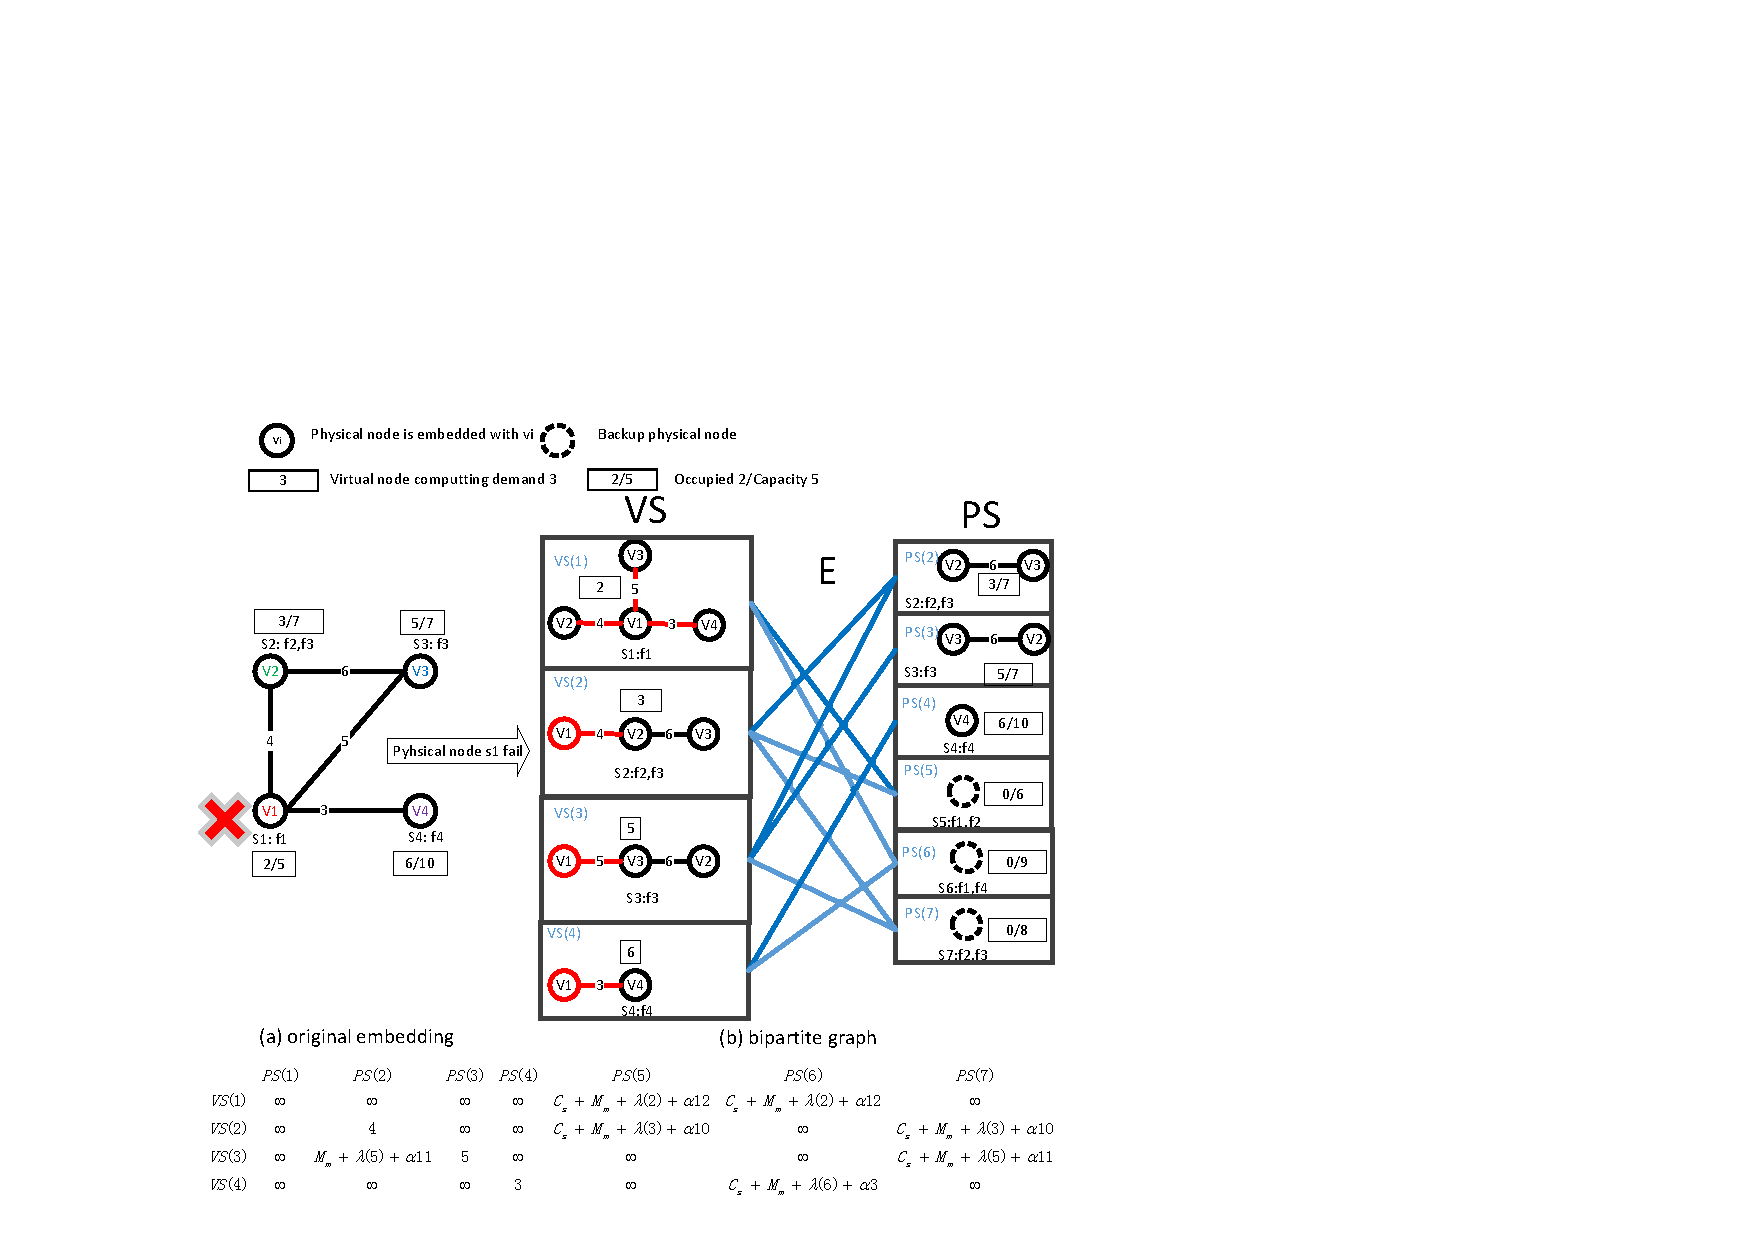
\includegraphics[width=3.7in]{Fig/StarRepresentation}\\
  \caption{Components of VirtualStar($v_i$) and PhysicalStar($s_j$) when physical node $s_1$ fail}\label{fig:StarRepresentation}
\end{figure}

\begin{equation*}
\tiny{
 {\begin{array}{*{20}{c}}
&R_{S_{1}}&R_{S_{2}}&R_{S_3}&R_{S_4}&R_{S_5}&R_{S_6}&R_{S_{7}}\\
{L_{V_1}}&\infty&\infty&\infty&\infty&\fbox{$C_{s}+M_{m}$+(2)+12}&C_{s}+M_{m}+(2)+12&\infty\\
L_{V_2}&\infty&\fbox{4}&\infty&\infty&C_{s}+M_{m}+(3)+10&\infty&C_{s}+M_{m}+(3)+10\\
L_{V_3}&\infty&M_{m}+(5)+11&\fbox{5}&\infty&\infty&\infty&C_{s}+M_{m}+(5)+11\\
L_{V_4}&\infty&\infty&\infty&\fbox{3}&\infty&C_{s}+M_{m}+(6)+3&\infty\\
\end{array}}
}
\label{lab:Node1FaliureAlignmentMatrixNew}
\end{equation*}


%\begin{equation*}
%\tiny{
% {\begin{array}{*{20}{c}}
%&{L_{V_1}}&L_{V_2}&L_{V_3}&L_{V_4}\\
%R_{S_{1}}&\infty&\infty&\infty&\infty\\
%R_{S_{2}}&\infty&\fbox{4}&M_{m}+(5)+11&\infty\\
%R_{S_{3}}&\infty&\infty&\fbox{5}&\infty\\
%R_{S_{4}}&\infty&\infty&\infty&\fbox{3}\\
%R_{S_{5}}&\fbox{$C_{s}+M_{m}$+(2)+12}&C_{s}+M_{m}+(3)+10&\infty&\infty\\
%R_{S_{6}}&C_{s}+M_{m}+(2)+12&\infty&\infty&C_{s}+M_{m}+(6)+3\\
%R_{S_{7}}&\infty&C_{s}+M_{m}+(3)+10&C_{s}+M_{m}+(5)+11&\infty\\
%\end{array}}
%}
%\label{lab:Node1FaliureAlignmentMatrixNew}
%\end{equation*}





For the virtual node $v_i$, if its virtual function can not be executed in physical node $s_j$
with $f(i) \notin F(i)$, no edge is connected with $VirtualStar(v_i)$ in $V_1$ and $PhysicalStar(s_j)$ in $V_2$. To facilitate problem formulation in following section, we set the edge weight to be $\infty $. For example, as $v_1$'s virtual function is $f_1$, it can not be executed in physical node $s_2$. Therefore, no edge is added to connected with $VirtualStar(v_1)$ in $V_1$ and $PhysicalStar(s_2)$ in $V_2$ and we set the $w(1,2)=\infty$.

For $VirtualStar(v_2)$, as $v_2$ is originally hold by $s_2$, however, when physical node $s_1$ (which holds $v_1$ originally) fails, the virtual link $e_{12}$ fails to be mapped to the physical network. We should find a new path connecting   $\phi(v_2)$ with $\phi(v_1)$ satisfying bandwidth demand  $d_{12}=4$. Therefore, the edge weight connecting $VirtualStar(v_2)$ and $PhysicalStar(s_2)$ is 4.

When node $s_1$ fails, it directly impact virtual node $v_1$. As $s_5$ can execute virtual function $f_1$, we can add a edge to  connect $VirtualStar(v_1)$ and $PhysicalStar(s_5)$. However, in this example, as $s_5$ does not setup virtual machine before, there also introduces virtual machine's start cost $C_s$.  Therefore, the link weight is $C_s$ (start cost)+ $M_m$ (migrating cost)+ $3$ (node capacity cost)+ $10$ (bandwidth cost).

\subsection{Problem formulation}
To provide survivable service, each virtual star (both the root virtual node and the virtual links connecting root node and its adjacent nodes) should be mapped to a physical star.
Assume virtual network consists of $n$ virtual nodes, thus $n$ virtual stars. The physical network consists of $m$ physical nodes, thus $m$ physical stars. In Eq(\ref{eq:indication}), we use bit binary $M_{ij}$ to denote whether  the $i$-th virtual star is mapped to the $j$-th physical star.
\begin{equation}
{M_{ij}} = \left\{ {\begin{array}{*{20}{c}}
   1 & {map \ virtualstar(i) \  to  \ physicalstar(j)}  \\
   0 & {otherwise}  \\
\end{array}} \right.
\label{eq:indication}
\end{equation}
When a physical node fails, to minimize the backup resource cost, the survivable virtual network embedding problem can be defined as follows.
\begin{equation}
\begin{array}{*{20}{c}}
   {\mathop {\min }\limits_{{M_{ij}}} } & {\sum\limits_{i = 1}^n {\sum\limits_{j = 1}^m {{M_{ij}}{w_{ij}}} } }  \\
   {s.t.,} & {\sum\limits_{i = 1}^n {{d_i}{M_{ij}}}  \le {c_j}}  \\
   {} & {\sum\limits_{j = 1}^m {{M_{ij}}}  \le 1}  \\
   {} & {{M_{ij}} = \{ 0,1\} }  \\
\end{array}
\label{eq:problem formulation}
\end{equation}
where ${\sum\limits_{i = 1}^n {\sum\limits_{j = 1}^m {{M_{ij}}{w_{ij}}} } }$ denotes the total backup resource  cost to map all the virtual stars to physical stars when physical nodes fails.  In (\ref{eq:problem formulation}), ${\sum\limits_{i = 1}^n {{d_i}{M_{ij}}}  \le {c_j}}$ is the physical node's capacity constraint, that is, even though multiple virtual nodes are allowed to be mapped to a physical node, the total capacity demand should not be larger than the capacity of the physical node. ${\sum\limits_{j = 1}^m {{M_{ij}}}  \le 1}$ indicates that one virtual star can be mapped to only one physical star.

Obviously, problem defined in (\ref{eq:problem formulation}) is an binary ILP problem, which is general an NP-complete problem according to Karp's 21 NP-complete problems\cite{karp1975computational}. %In following  Theorem 1, we validate the theorem.

\textbf{Theorem 1} Problem defined in (\ref{eq:problem formulation}) is an NP-complete problem.
\begin{proof}
If  there is only one physical node with $m=1$, our survivable virtual network embedding problem can be  degenerate into single knapsack problem, which is NP-complete problem. In practice, $m$ is usually larger than 1, single knapsack problem is subproblem of survivable virtual network embedding problem and given a feasible solution is easily verified in polynomial time, according to the reducibility theorem\cite{wood1987theory} in computer complexity field, it is easy to conclude that our defined in (\ref{eq:problem formulation}) is also NP-complete.
\end{proof}

\subsection{Dynamic Programming Mehtod}
\label{lab:DynamicProgrammingEquation}

Although solving the ILP formulation will result in a minimum cost survival virtual network embedding, its exponential time complexity makes such approach impractical to embed a virtual network to a large  physical network. In this section, we propose a dynamic programming based algorithm that has only a polynomial time complexity and, thus, is feasible for practical network systems.


To describe our dynamic programming based algorithm, we define  $dp[i][{x_1}][{x_2}] \ldots [{x_m}]$ to denote the best virtual star placement with the minimum backup resource cost to place the first $i$ ($0 \le i \le n $) virtual stars to the $m$ physical stars with their capacity  limit being $ x_1$, $ x_2$, $\ldots$, $x_m$ in the physical network.

The $i$-th virtual node star has the options to  be placed onto any one of the physical stars that are alive. Let $\theta (i,j)$ denote the backup resource cost to place the $i$-th virtual node star to the $j$-th physical node after the first $i-1$ virtual nodes are best placed. $\theta (i,j)$ is expressed as follows.
\begin{equation}
\footnotesize
\theta (i,j) = \left\{ {\begin{array}{*{20}{c}}
{dp[i - 1][x_1][{x_2}] \ldots [{x_j} - {d_i}] \ldots [{x_m}] + {w_{ij}}}\\
\infty
\end{array}} \right.\begin{array}{*{20}{c}}
{({x_j} \ge {d_i},{f_i} \in {F_j})}\\
{otherwise}
\end{array}
\label{eq:place i to j}
\end{equation}
In (\ref{eq:place i to j}), if the capability limit of the  physical node $x_j$ is large than the capacity demand $d_i$ and the virtual function $f_i$ can be executed in the physical node ${f_i} \in {F_j}$,  $\theta (i,j)$ is the sum of   the cost under best virtual star placement to place the first $i-1$ ($0 < i \le n $) virtual stars to the $m$ physical stars  (i.e., $dp[i-1][{x_1} - {d_i}][{x_2}] \ldots [{x_m}]$) and the cost that mapping the virtual star ($v_i$) to physical star ($s_1$) (i.e., $w_{i1}$ ).

Based on $\theta (i,j)$, $dp[i][{x_1}][{x_2}] \ldots [{x_m}]$ can be calculated through following dynamic programming function.
\begin{equation}
dp[i][{x_1}][{x_2}] \ldots [{x_m}] = min\{\theta (i,1),\theta (i,2),\ldots,\theta (i,j),\ldots,\theta (i,m)\}
\label{eq:update function}
\end{equation}


\begin{algorithm}
\label{alg:DPAlg}
\caption{Dynamic Programming Based Algorithm}
\begin{algorithmic}[1]
\REQUIRE {$dp[i][{x_1}][{x_2}] \ldots [{x_m}]=0(1\leq i \leq n, 0\leq x_1\leq c_1, 0\leq x_2\leq c_2,\ldots, 0\leq x_m\leq c_m)$ is firstly assigned as infinity $\infty$, $dp[0][{x_1}][{x_2}] \ldots [{x_m}]=0(0\leq x_1\leq c_1, 0\leq x_2\leq c_2,\ldots, 0\leq x_m\leq c_m)$, m is the number of physical nodes. $M[{x_1}][{x_2}] \ldots [{x_m}]=\textbf{0}_{n\times m}$ is placement of every virtual node.}
\ENSURE {obtaining optimal virtual node's placement when node up-bound capacity of physical nodes is $c_1,c_2,\ldots,c_m$, respectively.}
\FORALL{$i$ such that $1\leq i\leq n$ }
\FORALL{$x_1,x_2,\ldots,x_m$ such that $ c_1\geq x_1\geq d_i$, $c_2\geq x_2\geq d_i$,$c_3\geq x_3\geq d_i$,$c_m\geq x_m\geq d_i$}

\STATE {$dp[i][{x_1}][{x_2}] \ldots [{x_m}] = min\{\theta (i,1),\theta (i,2),\ldots,\theta (i,j),\ldots,\theta (i,m)\}$}

\STATE{$j' = \mathop {\arg \min }\limits_j \{\theta (i,1),\theta (i,2),\ldots,\theta (i,j),\ldots,\theta (i,m)\}$, }.
\STATE{$M[{x_1}][{x_2}] \ldots [{x_m}]=M[{x_1}][{x_2}] \ldots[x_{j'}-d_i]\ldots [{x_m}]$}
\STATE{$M[{x_1}][{x_2}] \ldots [{x_m}]_{ij'}=1$}
\ENDFOR
\ENDFOR
\RETURN $dp[i][{c_1}][{c_2}] \ldots [{c_m}]$ and $M[{c_1}][{c_2}] \ldots [{c_m}]$
\end{algorithmic}
\end{algorithm}

%\left[ {\begin{array}{*{20}{c}}
%0&0&0&0&0&0&0\\
%0&0&0&0&0&0&0\\
%0&0&0&0&0&0&0\\
%0&0&0&0&0&0&0
%\end{array}} \right]
The pseudo-code of the dynamic programming based algorithm is shown in Alg.\ref{alg:DPAlg}.
We further use an example in Fig.\ref{fig:DPIllustration} to illustrate the algorithm.

For clear presentation, in this example, three virtual stars needed to be placed to two available physical stars to achieve the minimum backup resource cost. The available capacity under physical nodes are $c_1=5$ and $c_2=4$, respectively. The capacity demands of these three virtual stars are $d_1=2$, $d_2=1$, and $d_3=2$. The virtual functions required to be executed in these virtual stars are $f(1)=f_1$, $f(2)=f_1$, $f(3)=f_2$. The functions supported by these two physical nodes are $F(1)=\{f_1,f_2\}$ and $F(2)=\{f_1\}$.

In Fig.\ref{fig:DPIllustration}, $x$ and $y$ axis denote the capacity limit of physical star $s_1$ and $s_2$, respectively. The  weight of edge connecting virtual stars to physical stars are $w_{11}=1$, $w_{12}=2$, $w_{21}=3$, $w_{22}=1$, $w_{31}=1$, $w_{32}=\infty$, respectively.


Initially, in Fig.\ref{fig:DPIllustration}(a), as no virtual star is placed to any physical stars, the backup cost under all the capacity limit cases ($x_1$=0,1,2,3,4 and $x_2$=0,1,2,3,4,5) are all 0. Specially, even though capacity limits are set 4 and 5, dp[0][4][5]=0.

In Fig.\ref{fig:DPIllustration}(b), when place the first virtual node $v_1$ with capacity demand $d_1=1$ to these two physical nodes, as $f_1$ can be executed in both physical nodes. Therefore, we have
\begin{equation}
dp[1][{x_1}][{x_2}] = \min \{\theta (1,1),\theta (1,2)\}
\end{equation}
Specially, if the capacity limit of these two physical nodes are $x_1$=2 and $x_2$=0, we have $dp[1][2][0]= dp[0][0][0]+w_{11}=2$. If the capacity limit of these two physical nodes are $x_1$=2 and $x_2$=4, we have $\theta (1,1)=dp[0][0][2]+w_{11}$ and $\theta (1,2)=\infty$ and thus $dp[1][2][4]=min\{ dp[0][0][4]+w_{11}), dp[0][2][2]+w_{12} \}=1$.

Similarly, when place the second virtual node with capacity demand $d_2=2$ to these two physical nodes, the cost results under all capacity limits is shown in Fig.\ref{fig:DPIllustration}(d). As $f_2$ can be executed in both physical nodes, thus $v_2$ can be placed into both physical nodes, we have
\begin{equation}
dp[2][{x_1}][{x_2}] = \min \{\theta (2,1),\theta (2,2)\}
\end{equation}
Specially, if the capacity limit of these two physical nodes are $x_1$=3 and $x_2$=4, we have $dp[2][3][4]=min\{dp[1][2][4]+w(2,1), dp[1][3][3]+w(2,2)\}=2$. If the capacity limit of these two physical nodes are $x_1$=3 and $x_2$=0, we have $dp[2][3][0]=dp[1][2][0]+w(2,1)=4$.

Fig.\ref{fig:DPIllustration}(d) shows the minimum resource cost result  when  place the third virtual node with capacity demand $d_3=1$ to these two physical nodes. As $f_3$ can only be executed in physical node $s_1$, we have $\theta (3,2)=\infty$. Specially, if the capacity limit of these two physical nodes are $x_1$=5 and $x_2$=0, we have $dp[3][5][0]=dp[2][3][0]+w(3,1)=4$. As the node capability of these two physical nodes are 5 and 4, respectively, we have $dp[3][5][4]=dp[2][3][4]+w(3,1)=3$, as indicted in Fig.\ref{fig:DPIllustration}(d), the best placement is achieved at dp[3][5][4]=3 with the assignment $v_1\rightarrow s_1, v_2\rightarrow s_2, v_3\rightarrow s_1$.

For example, as shown in Fig.\ref{fig:StarRepresentation} and Equ.(\ref{lab:Node1FaliureAlignmentMatrixNew}), the optimal $M_{ij}=\left[ {\begin{array}{*{20}{c}}
0&0&0&0&1&0&0\\
1&0&0&0&0&0&0\\
0&1&0&0&0&0&0\\
0&0&1&0&0&0&0
\end{array}} \right]$.

\begin{figure}
\centering
% Requires \usepackage{graphicx}
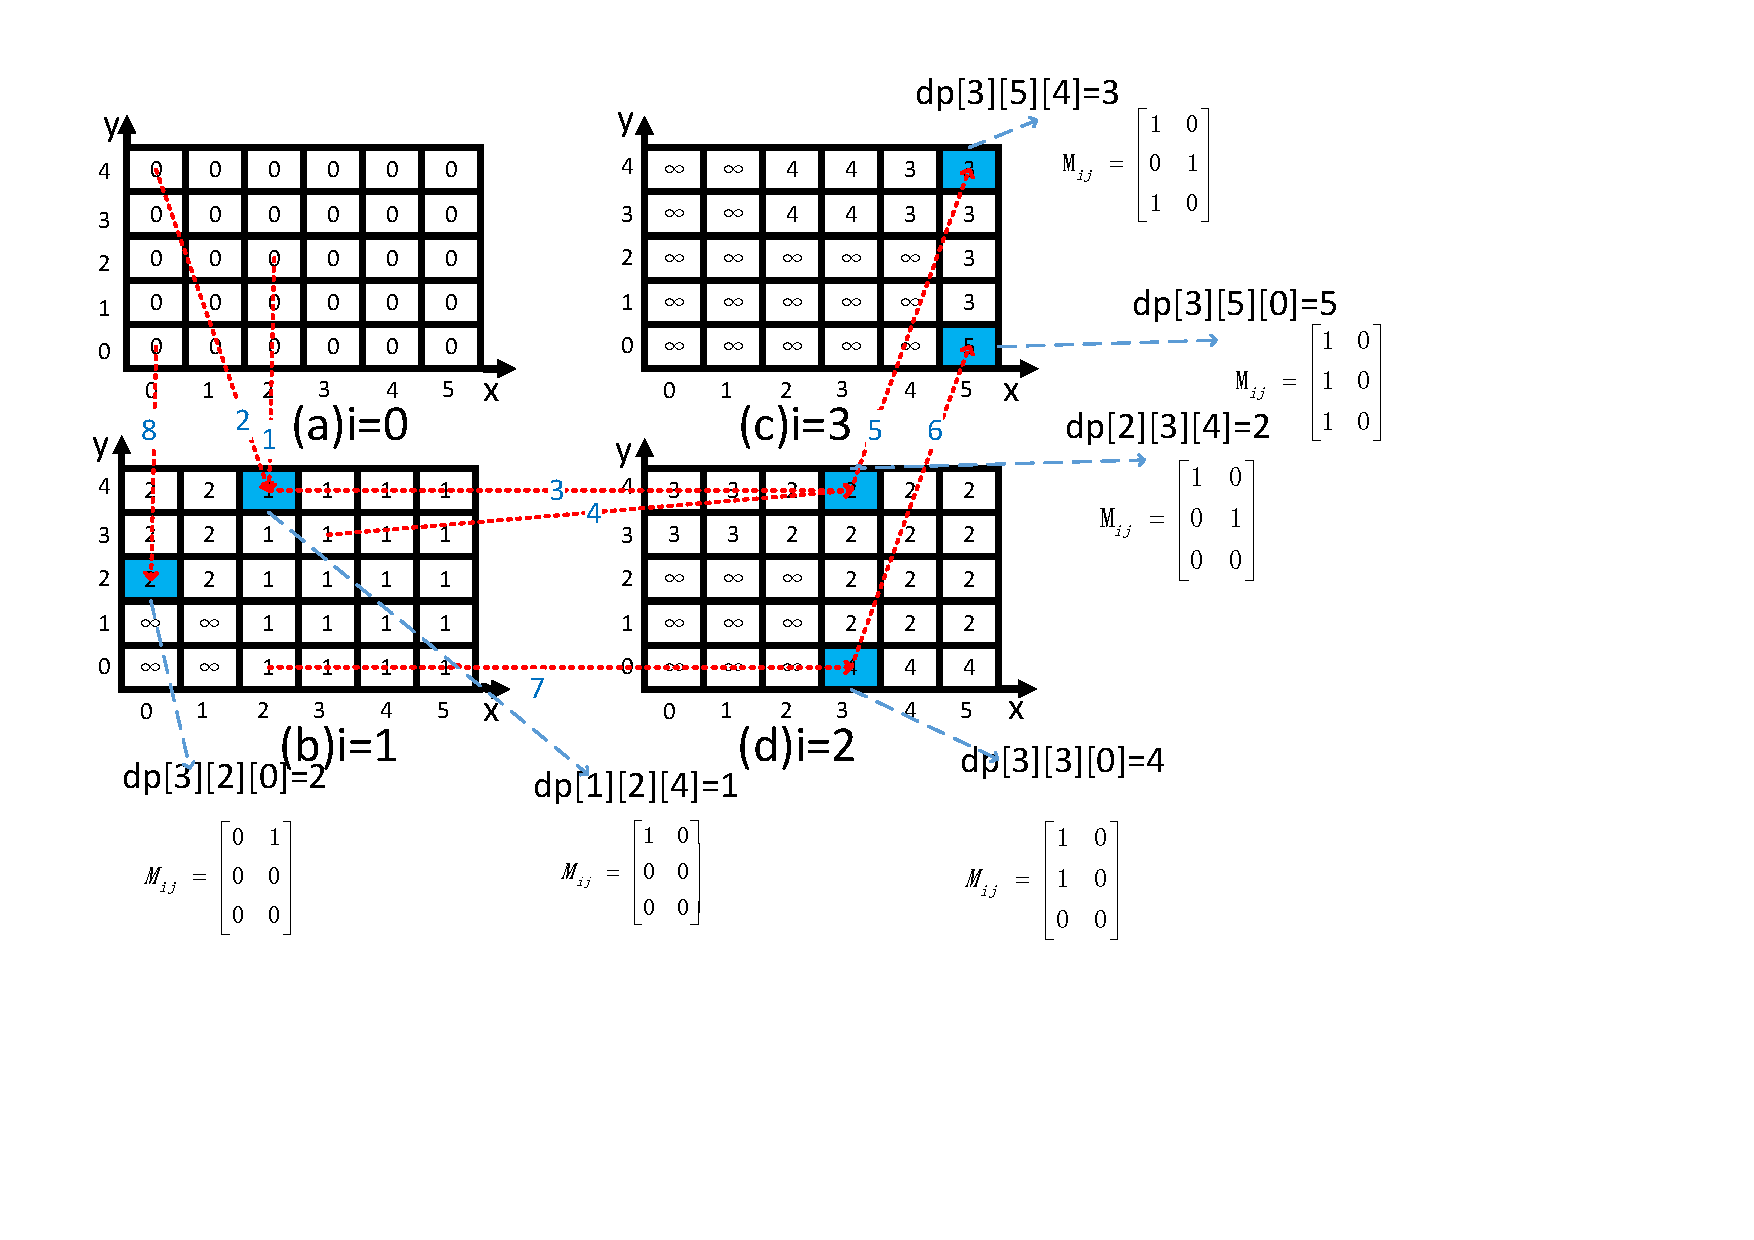
\includegraphics[width=4in]{Fig/DPIllustration}\\
  \caption{Three virtual node, the first virtual node could be placed to first and second physical node,  the second virtual node could be placed to first and second physical node,  the third virtual node could only be placed to first physical node.  The  node computation capacity of first physical node is 5, the node computation capacity of second physical node is 4. $w_{ij}$=[1,2;3,1;1,$\infty$].}\label{fig:DPIllustration}
\end{figure}




\begin{figure}
\centering
% Requires \usepackage{graphicx}
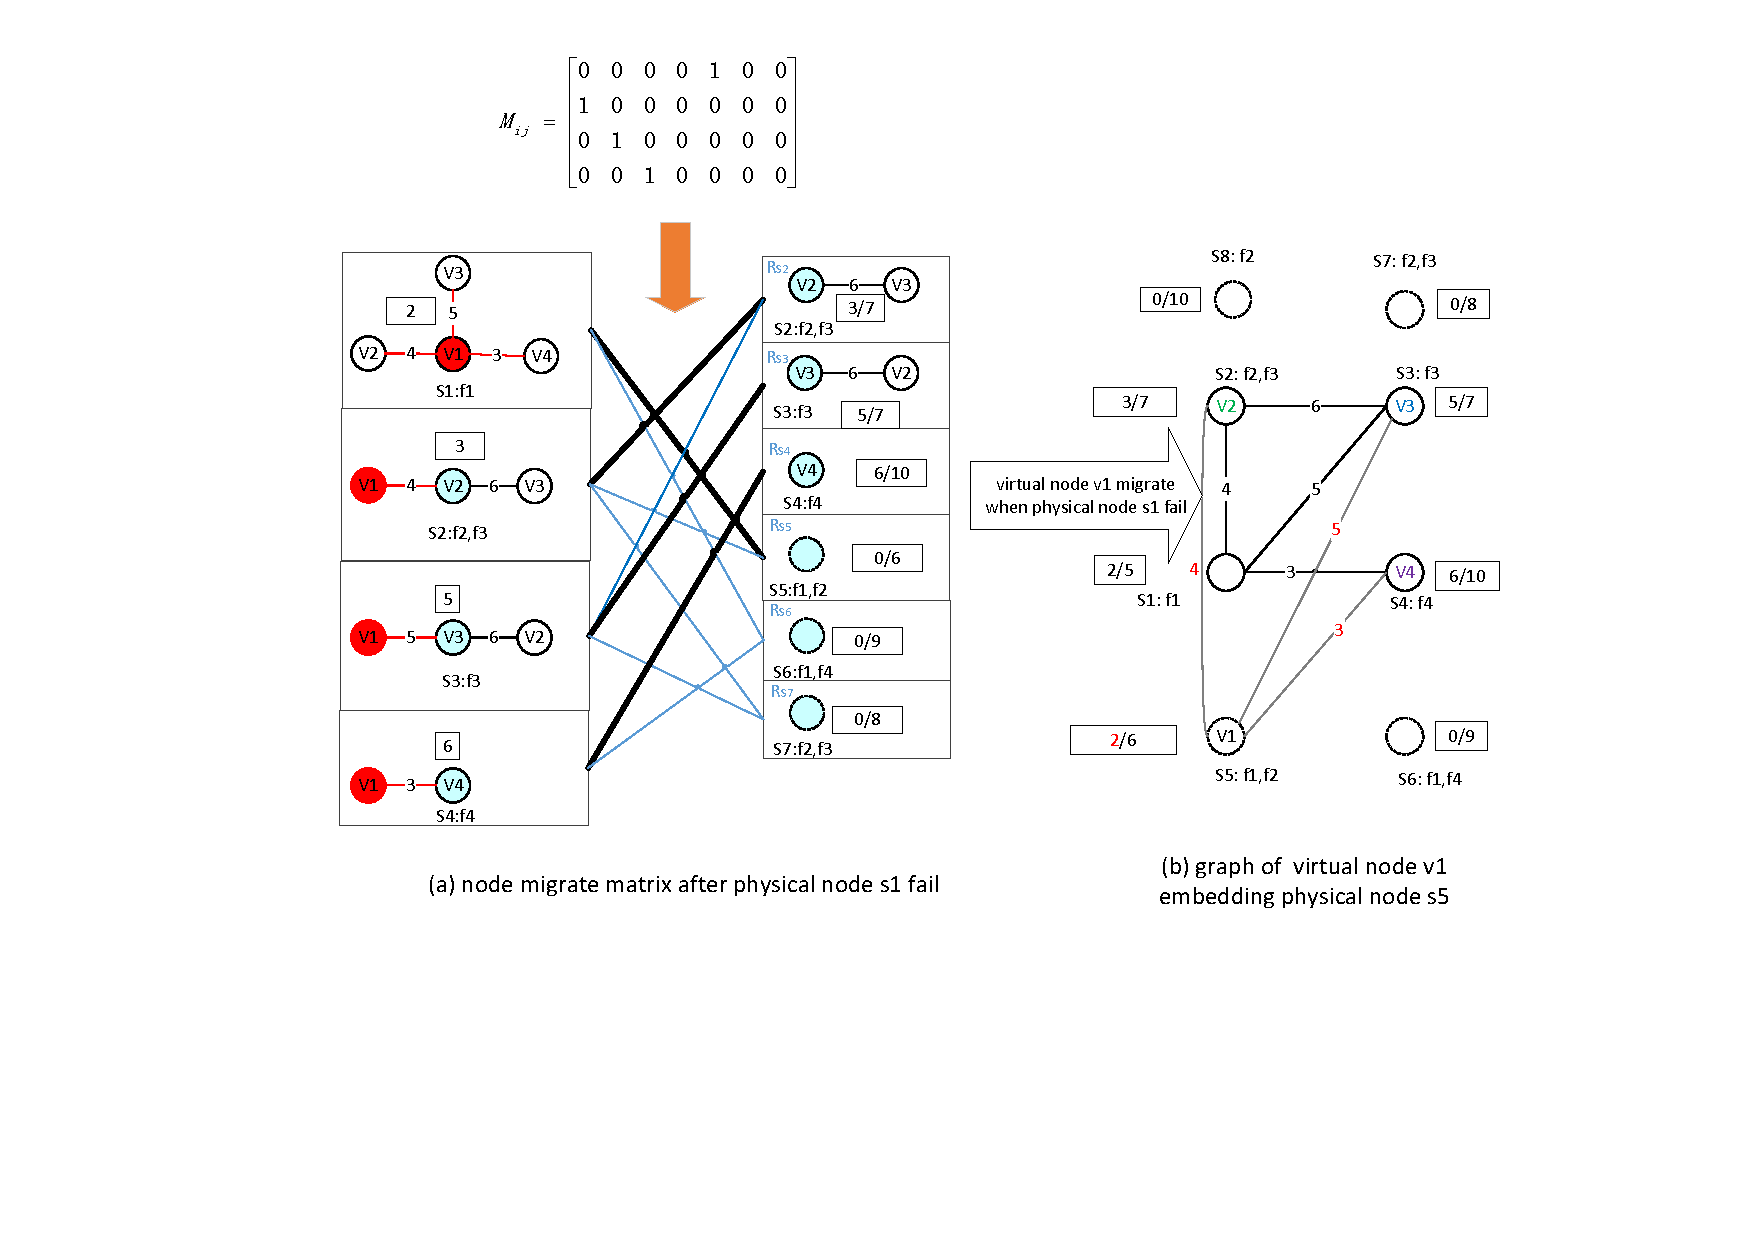
\includegraphics[width=4in]{Fig/Node1Failure}\\
  \caption{Node1Failure}\label{fig:Node1Failure}
\end{figure}

\begin{figure}
\centering
% Requires \usepackage{graphicx}
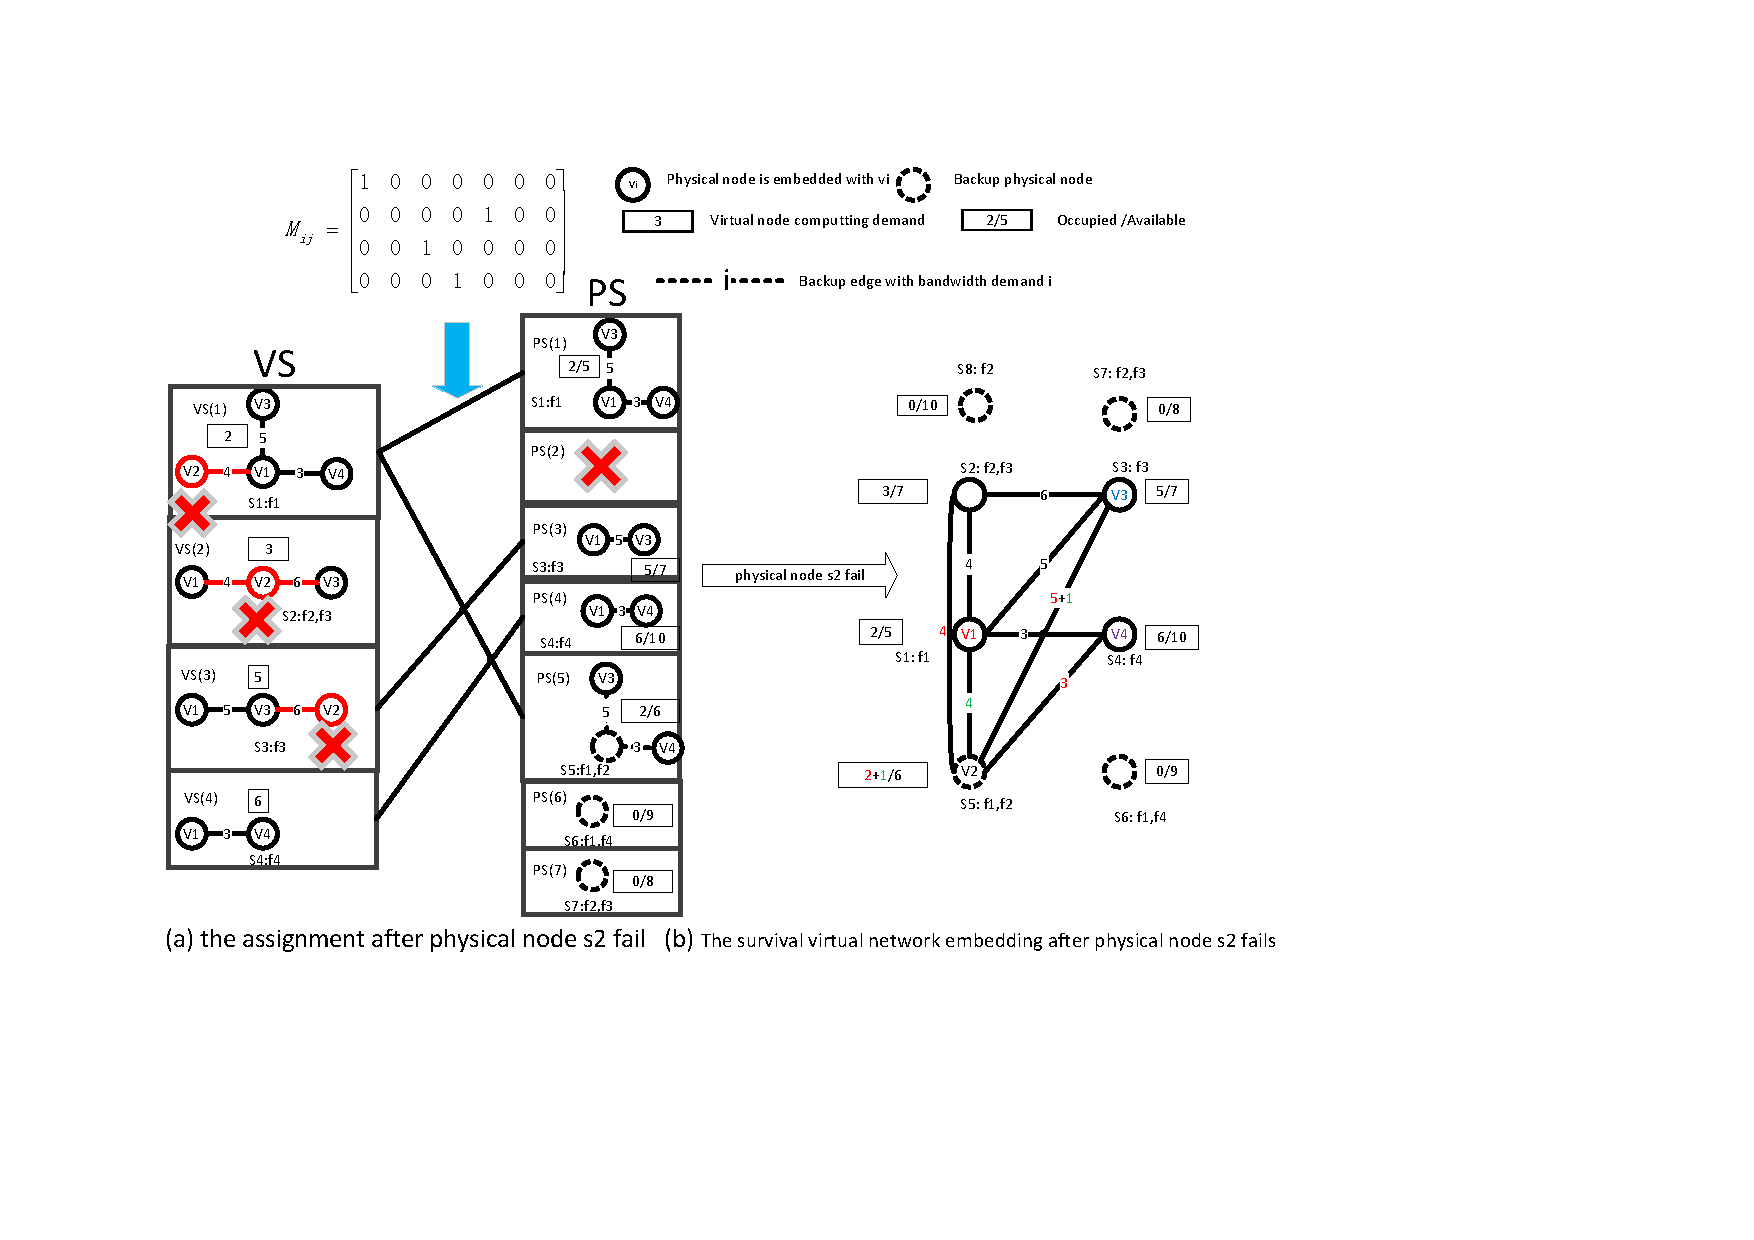
\includegraphics[width=4in]{Fig/Node2Failure}\\
  \caption{Node2Failure}\label{fig:Node2Failure}
\end{figure}

\begin{figure}
\centering
% Requires \usepackage{graphicx}
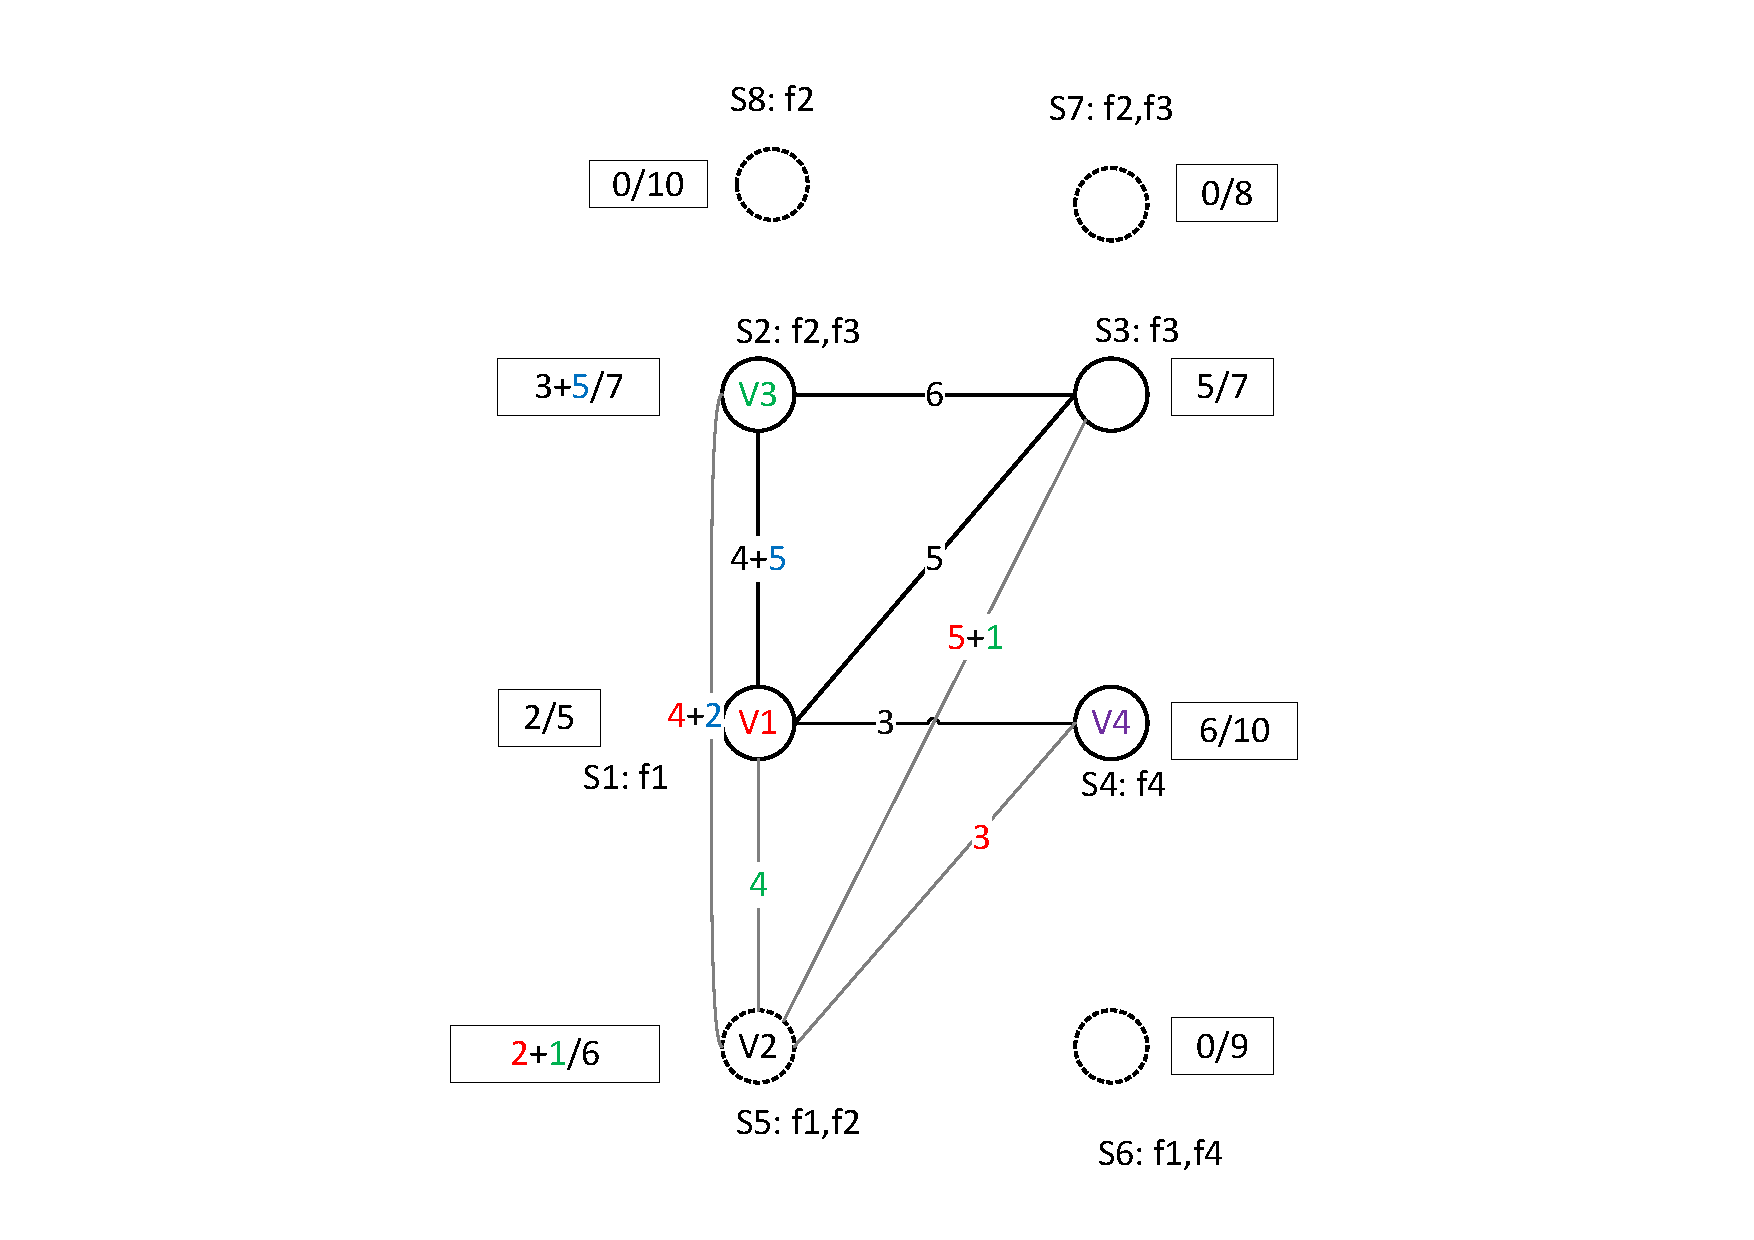
\includegraphics[width=2in]{Fig/Node3Failure}\\
  \caption{Node3Failure}\label{fig:Node3Failure}
\end{figure}

\begin{figure}
\centering
% Requires \usepackage{graphicx}
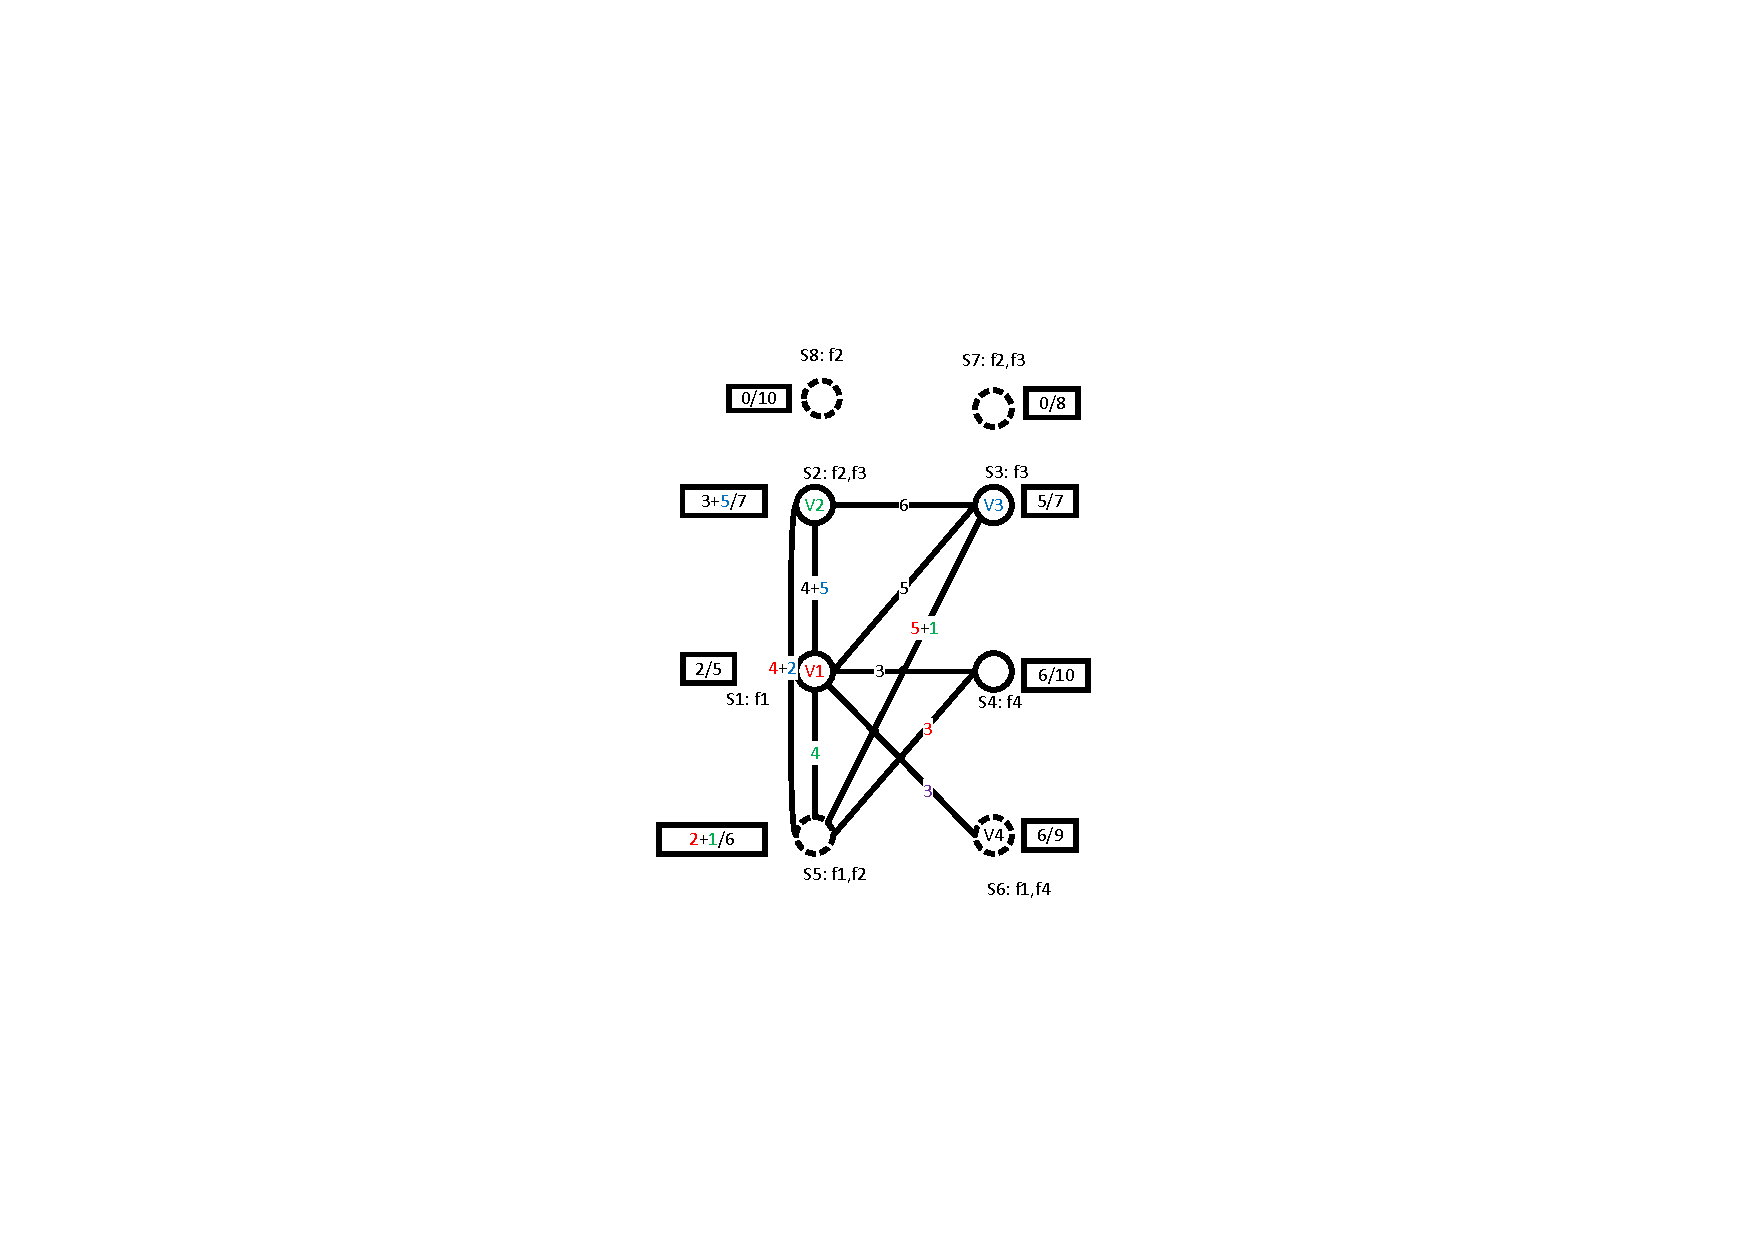
\includegraphics[width=2in]{Fig/Node4Failure}\\
  \caption{Node4Failure}\label{fig:Node4Failure}
\end{figure}










